\documentclass{article}
\usepackage{amsmath}
\usepackage{amssymb}
\usepackage{graphicx}

\newcounter{probcnt}
\newenvironment{problem}{\stepcounter{probcnt}{\bf Problem \arabic{probcnt}}.}{}
\setlength{\parskip}{.3cm}
\setlength{\parindent}{0cm}


\title{CS 440 / ECE 448: Introduction to AI \\ HW 1}
\date{\vspace{-0.4in}Due: Tuesday,  February 4, 2014}
\begin{document}
\maketitle

\emph{Your answers must be concise and clear. Explain sufficiently that we can easily determine what you understand. We will give more points for a brief interesting discussion with no answer than for a misleading answer.}

\emph{Assignments must be submitted via Compass 2g, in PDF. You are strongly encouraged to edit your answers in LaTeX. Do not submit handwritten solutions.}

\begin{problem}{}
Consider the search tree in Figure \ref{st}. Node $A$ is the root of the tree and the double circled nodes are the goal states. The number inside each node represents the value of the heuristic for that node, $h(n)$. The number by each edge represents the cost of traversing the edge.

\begin{figure}
\caption{Search tree}
\center{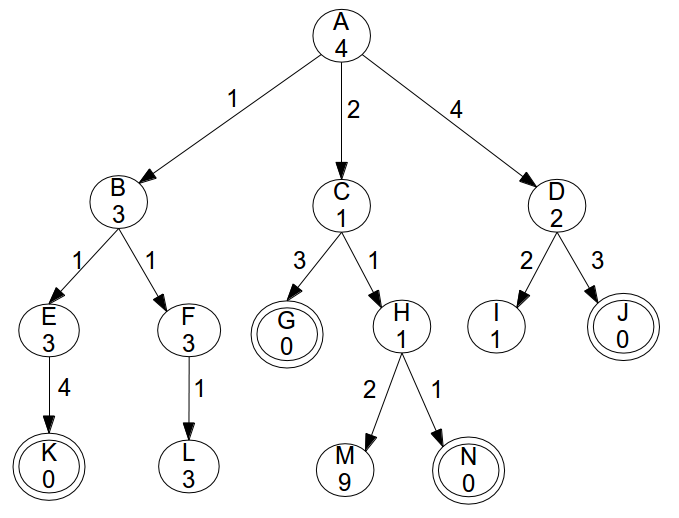
\includegraphics[scale=0.3]{st-ex-o}}
\label{st}
\end{figure}

\begin{enumerate}
\item[(a)] For each of the search strategies below, show the order in which the nodes are visited, the state of the queue at each step of the search, the goal state found (if any), and whether or not this goal state is optimal. New nodes are added to the queue in alphabetical order whenever the order is indifferent for the search algorithm.
	\begin{enumerate}
	\item[(i)] depth-first 
	\item[(ii)] breadth-first 
	\item[(iii)] uniform-cost 
	\item[(iv)] greedy/best-first
	\item[(v)] $A^*$
	\end{enumerate}

\item[(b)] For each of these search strategies say whether it is admissible.  Explain your answers.
	
\item[(c)] Assume the path cost from any state to an unreachable state is infinite. Is the heuristic consistent? Explain your answer. 
\end{enumerate}
\end{problem}

\begin{problem}{}
Consider the grid world in Figure \ref{gw}. The numbers in the squares mark the elevation. The agent's objective is to have both boxes, initially in the squares marked as 'Box', in the same square. The agent's initial position is the north-east corner of the grid. It can carry at most one box at a time. The actions available are:
	\begin{itemize}
		\item \emph{Pick Up}: the agent picks up a box in the current square, if there is one
		\item \emph{Drop}: the agent drops a box in the current square, if carrying one
		\item \emph{Move South}: the agent takes a step south if possible
		\item \emph{Move North}: the agent takes a step north if possible
		\item \emph{Move East}: the agent takes a step east if possible
		\item \emph{Move West}: the agent takes a step west if possible
	\end{itemize}

Moving into any of the walls (outer edges of the grid) results in the same square as before attempting movement.

The cost of picking up a box is 5, whereas the cost of dropping a box is 1. The cost of moving from square a to square b is $\max (1, 10-(e(a)-e(b)))$ if the agent is not carrying a box, and $\max (1, 10-2*(e(a)-e(b)))$ if the agent is carrying a box, where $e(a)$ denotes the elevation of square $a$.

\begin{figure}
\centerline{
\begin{tabular}{|c|c|}
\hline
& Start \\
9 & 7 \\
& \\
\hline 
Box & Box \\
10 & 1 \\
 & \\
\hline
\end{tabular}
}
\caption{Grid world}
\label{gw}
\end{figure}
\begin{enumerate}
	\item[(a)] \begin{enumerate}
		\item[(i)] Define a simple data structure sufficient to represent the states for this problem. What does a goal state look like in your representation?
		\item[(ii)] Define the operators \emph{Pick Up} and \emph{Drop} by specifying their preconditions and effects	
	\end{enumerate}
	\item[(b)] Suppose the robot is allowed to choose the order in which it adds the successors of the expanded node to the queue, in each step, during search, when this order is indifferent to the specific search algorithm.
	\begin{enumerate}
		\item[(i)] What is the fewest possible number of nodes that must be visited if breadth-first search is performed? Is it guaranteed to reach the goal state? Would an optimal solution be found?
		\item[(ii)] What is the fewest possible number of nodes that must be visited if depth-first search is performed? Is it guaranteed to reach the goal state? Would an optimal solution be found?
		\item[(iii)]  What is the fewest possible number of nodes that must be visited if uniform-cost search is performed? Is it guaranteed to reach the goal state? Would an optimal solution be found?  
	\end{enumerate}
\end{enumerate}
\end{problem}

\begin{problem}
Consider function $f:[0,1]^3\to \mathbb{R}$ with the following form:
\[
f(x,y,z)=x\cdot \ln x + y \cdot \ln y + z \cdot \ln z + \alpha \cdot (x + y + z - 1)
\]
where $\alpha > 0$
\begin{enumerate}
	\item[(a)] Compute the gradient of the function. Show your work. 
	\item[(b)] For $\alpha=1$, compute the value of the gradient at these points: 
	
	$(0.9,0.4,0.01);(0.7,0.2,0.04);(0.1,0.12,0.14)$
	\item[(c)] Compute the Hessian of the function. Show your work.
	\item[(d)] Is this function convex, concave, or neither? Explain.
	\item[(e)] Is the domain of the function convex? Explain.
	\item[(f)] Compute the optima of the function and say, for each point, whether it is a minimum or a maximum. Show your work.
\end{enumerate}
\end{problem}

\end{document}
